\documentclass[11pt]{article}

\usepackage[margin=1in]{geometry}
\usepackage[utf8]{inputenc}
\usepackage[T1]{fontenc}
\usepackage{lmodern}
\usepackage{amsmath,amssymb,amsthm}
\usepackage{booktabs}
\usepackage{microtype}
\usepackage[numbers,sort&compress]{natbib}
\usepackage{xcolor}
\usepackage{tikz}
\usetikzlibrary{arrows.meta,positioning,fit,calc}
\usepackage[colorlinks=true,linkcolor=blue!50!black,citecolor=blue!50!black,urlcolor=blue!50!black]{hyperref}

\newcommand{\draftnote}[1]{\textcolor{red!70!black}{[\textbf{Draft:} #1]}}

\title{One Window, Two Functions:\\Where Certified Transducer Learning Stops, and Separate Paths\\for the Transition and the Output\\[0.5em]
\large Research note, 19 October 2026: not for circulation}

\author{
  David Barkhuizen\\
  Independent researcher
  \and
  Claude (Opus 5.5)\\
  Anthropic
}

\date{}

\begin{document}

\maketitle

\draftnote{A stand-alone note of the work of 18--19 October 2026, written at the first author's
request. Its numbers come from \texttt{indrajala-ml}'s recorded findings (the docstring of its
probe script, \texttt{modular\_family\_probe.py}, and the workplans under \texttt{docs/}),
at the commits and pull requests named in Section~\ref{sec:provenance}. Its material may move into
the two papers (\texttt{snapped-window-recurrence.tex}, \texttt{certified-modular-division.tex})
once the window-branches experiments read out.}

\begin{abstract}
Our method learns a finite-state transducer from input--output examples and certifies the learned
machine exactly. Tested at its limits, it certifies modular division at 121 states but not at 169,
and fails on the symmetric group's word problem and move-to-front at 120 states. Neither a three
times longer training budget, a wider state, nor four remedies aimed at retaining near solutions
moves those limits. Diagnosing the nearest failure at 169 states, we find its state machine
\emph{exactly right}: the error is in the answers. Its answers are read linearly from the same
16-wide features that every factor of the state reads, and those features don't linearly separate
the answers: a readout fitted to convergence on all 2{,}025 (state code, input) pairs still gets 6
wrong. A Mealy machine is two functions, the transition $\delta$ and the output $\lambda$. Our
window computes both from one representation. We propose giving each a path of its own (and each
state factor its own), and register the claims that test it.
\end{abstract}

\section{Setting}

The method (\texttt{snapped-window-recurrence.tex}) trains a window-recurrent network: a small
causal transformer reads a window of input tokens and the current state, and the state is
\emph{factored} into $G$ parts, each part's next value snapped to the nearest of a learned
codebook (vector quantisation with a straight-through gradient). Each factor $g$ has its own
attention pooling (one learned query, one head) over the window's output tokens, its own gated
cell and its own codes. Because the state is finite, the trained network \emph{is} a finite-state
machine, which we read out and compare with the target transducer exactly: a \emph{certificate}
checks every reachable state code against every input, and passes only with no wrong output, no
wrong next state, and margins above a tolerance. We require both verdicts (the default snap-ratio
tolerance and the strict 1.0). Training follows a curriculum of lengths, with a \emph{fork} that
restores the network after a collapse, and every cell is feasible: the codes can represent the
target's minimal states, and the training lengths exceed the exclusion bound $m + q - 1$ ($m$ the
joint codes, $q$ the target's states) below which a wrong machine can fit every training word.
Each cell runs seeds 0--5; a cell \emph{works} if any seed certifies, and 0 of 6 against 4 of 6
is Fisher one-sided $p = 0.030$. Every claim below was registered before its data.

The window (W11) is three transformer blocks, each after a \texttt{StateInput} that adds a
projection of the whole state to every token, writing one residual stream of width $D = 16$ per
token, 2 attention heads per block and a feed-forward width of 32. The answers are a single linear
layer over the final tokens, and every factor's pooling reads the same final tokens.

\section{Where the method stops}
\label{sec:limits}

\paragraph{Modular division (a ladder in $p$).} Division mod $p$ is a $p^2$-state transducer.
With $p$~11's cell (two factors of width 16, $\lceil 32p/11 \rceil$ codes each), only $p$ changed:

\begin{center}
\begin{tabular}{lrrrl}
\toprule
$p$ & states & epochs & certified & worst answer at best \\
\midrule
11 & 121 & 600 & 4 of 6 & -- \\
13 & 169 & 600 & 0 of 6 & 0.394--0.916 \\
13 (three times the budget) & 169 & 1{,}800 & 0 of 6 & 0.394--0.936 \\
13 (each factor 32 wide) & 169 & 600 & 0 of 6 & 0.382--0.994 \\
17 & 289 & 600 & 0 of 6 & 0.609--0.774 \\
23 & 529 & 600 & 0 of 6 & 0.360--0.386 \\
\bottomrule
\end{tabular}
\end{center}

The edge lies between 121 and 169 states, and it is neither the budget (the first 600 of the
1{,}800 epochs repeat the 600-epoch runs by bits, across machines, and the extra epochs add
nothing) nor the state's width. Widening each factor from 16 to 32 dimensions moved the runs,
descriptively: four of six formed a state at their best step (a state share of 0.996--1.0, against
two of six at width 16), and one (seed 5) minimised to 172 states against 169.

\paragraph{The general algebras at 120 states.} The word problem of the symmetric group $S_5$ (a
group: every input a permutation) and move-to-front on five items (aperiodic), each 120 states, in
the same cell as $p$~11 (32 codes a factor): 0 of 6 each. So both Krohn--Rhodes extremes fail at
120 states while division certifies at 121: the state count alone is not the limit. Two mechanisms,
both seen at smaller sizes. \emph{Extra codes}: $S_5$'s runs formed an exact core (each state's
first code breaking 0--4\% of its transitions) but reached 385--748 codes, whose transitions break,
and minimised to 175--842 states. \emph{Failure A}: four of move-to-front's runs never formed a
state (2--3 codes a factor).

\paragraph{Retention remedies.} Every failing run near a solution lost it. Four remedies, each a
registered probe, found no gain: consolidating codes the network itself can't tell apart, longer
training words, and restoring each curriculum step's best network all certified 0 of 6 on a
16-state random machine. The certificate guard, which undoes any update that breaks a machine
already right, made things worse on move-to-front at 24 states (1 of 6 guarded against 3 of 6
unguarded; the symmetric group's $S_4$ 6 of 6 in both). It arms on a perfect screen, which isn't a
certificate. Two networks it armed on were right at snap ratio 1.0 but had 6--8 near ties at the
default tolerance. Holding them, the guard undid 96\% and 100\% of the updates until a stall rule
ended the runs, where unguarded the same seeds certified within 1--3 steps.

\paragraph{The commitment and failure A (partial).} With the codebook's commitment term off for
the curriculum's first five steps, three of round~1's six failure-A runs formed a state by step 5's
end (shares 0.87, 0.97, 1.0, against at most 0.38 with it on), and one certified. That meets the
registered answer: the commitment's pull causes failure A. When the commitment returned, the
states eroded (0.97 to 0.43; 0.87 to 0.67). Four of the six runs were stopped by the first author
at 516--558 of their 600 epochs, after the registered reading (step 5) was complete.

\section{The diagnosis at 169 states}
\label{sec:diagnosis}

The nearest failure, division $p$~13 with factors 32 wide (seed 5's best network), passes every
transition: \textbf{0 wrong states in both verdicts}. It fails on 22 outputs, and those wrong
outputs are what make three states look distinct (172 against 169).

\paragraph{The readout alone.} The poolings read the input of the output layer, so that layer
affects only the answers. Training it alone (every other parameter frozen, tested bit for bit),
the machine minimised to exactly 169 states after one epoch, but 15--19 wrong outputs remained for
29 more epochs. They are confident (logit leads up to 4.3) and on the states' own first codes, over
12 of the 169 states.

\paragraph{Separability.} We read the 16 features the output layer reads, at the quotient's
position, for every reachable code and input: 225 codes $\times$ 9 inputs $=$ 2{,}025 pairs. An
unregularised softmax readout fitted to all of them (full batch, 60{,}000 Adam steps) went from 17
wrong to 6 by step 20{,}000 and stayed at 6. A multiclass perceptron, which reaches zero errors in
finitely many passes on linearly separable data, never got below 6 in 20{,}000 passes. For each of
the six, a feature vector with a \emph{different} answer lies nearer than any with the same answer:

\begin{center}
\begin{tabular}{rrrrrr}
\toprule
target state & input & answer & nearest answer & distance to it & nearest same answer \\
\midrule
57 & 2 & 3 & 4 & 0.364 & 0.455 \\
76 & 5 & 9 & 2 & 0.384 & 0.883 \\
64 & 6 & 4 & 3 & 0.322 & 0.686 \\
134 & 3 & 8 & 2 & 0.331 & 0.633 \\
135 & 3 & 9 & 2 & 0.504 & 0.647 \\
148 & 5 & 2 & 8 & 0.333 & 0.335 \\
\bottomrule
\end{tabular}
\end{center}

So no linear readout of the window's features certifies this network, however it is trained (strong
evidence rather than proof: a perceptron's non-convergence is not one). Two further readings
follow. Sampled training was part of the readout's failure (fitted on every pair, 15 errors fall to
6). And the remaining errors are a property of the features themselves.

\section{One window, two functions}
\label{sec:design}

A Mealy machine is a pair of functions of the state $q$ and the input $a$: the transition
$\delta(q, a)$ and the output $\lambda(q, a)$. Our window computes both from one representation:
16 numbers a token carry what each factor's pooling needs for $\delta$ and what a linear map needs
for $\lambda$ over $169 \times 9$ (state, input) pairs. The diagnosis above is what that sharing
predicts. The learned $\delta$ is exact, and $\lambda$'s pairs collide in the shared features.

The first author conjectured the remedy: one attention head per factor (per codebook) and one for
the answers. We make it a design, \emph{window branches} (Figure~\ref{fig:branches}). The window's
first two blocks stay a shared trunk, which reads the columns and the state for every consumer.
Its last block is replaced by one block per consumer, each with one attention head and its own
feed-forward layer: one branch for each factor's pooling, and one for the answers. Every path keeps
the window's depth of three blocks, so the comparison with today's window changes the separation,
not the depth. The answers' branch can then be trained alone after the state is right, without
risk to it. And the design mirrors the transducer, factored per state component and split between
$\delta$ and $\lambda$.

\begin{figure}[t]
\centering
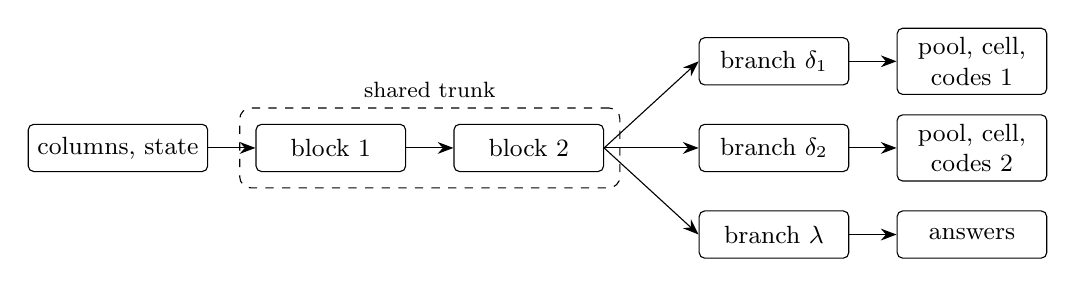
\begin{tikzpicture}[
  box/.style={draw, rounded corners=2pt, minimum height=6mm, minimum width=19mm, font=\small, align=center},
  arr/.style={-{Stealth[length=2mm]}},
  node distance=4mm and 6mm]
\node[box] (in) {columns, state};
\node[box, right=of in] (b1) {block 1};
\node[box, right=of b1] (b2) {block 2};
\node[box, right=12mm of b2, yshift=11mm] (f1) {branch $\delta_1$};
\node[box, right=12mm of b2] (f2) {branch $\delta_2$};
\node[box, right=12mm of b2, yshift=-11mm] (ans) {branch $\lambda$};
\node[box, right=of f1] (p1) {pool, cell,\\ codes 1};
\node[box, right=of f2] (p2) {pool, cell,\\ codes 2};
\node[box, right=of ans] (out) {answers};
\draw[arr] (in) -- (b1); \draw[arr] (b1) -- (b2);
\draw[arr] (b2.east) -- (f1.west); \draw[arr] (b2.east) -- (f2.west); \draw[arr] (b2.east) -- (ans.west);
\draw[arr] (f1) -- (p1); \draw[arr] (f2) -- (p2); \draw[arr] (ans) -- (out);
\node[draw, dashed, rounded corners, fit=(b1)(b2), inner sep=2mm, label={[font=\footnotesize]above:shared trunk}] {};
\end{tikzpicture}
\caption{Window branches with two state factors. Today's window has a third shared block whose
tokens both poolings and the answers read; here each consumer has its own single-head block.}
\label{fig:branches}
\end{figure}

\paragraph{Registered claims} (\texttt{docs/window-branches-workplan.md}, before their data). The
branches are built whatever these find; the claims decide whether they become the default window.
\begin{itemize}
\item \textbf{W1, width alone}: $p$~13 with factors 32 wide and the window's stream 32 wide instead
  of 16, against the 0 of 6 above. If it works, a crowded 16-wide stream limited division at 13.
  (Running at the time of writing. The default width repeats the earlier runs by bits on the new
  code.)
\item \textbf{B1}: the branches on the same cell, at width 16, against the same 0 of 6.
\item \textbf{B2}: the branches on $S_5$ and move-to-front at 120 states, against 0 of 6 each.
\item \textbf{B3, no harm}: the branches on division $p$~11 and on $S_4$ and move-to-front at 24
  states, each 4 of 6 today. Harm is 0 of 6 on any of them.
\item \textbf{Adoption}: the branches become the default if B1 or B2 works where its control failed
  and B3 shows no harm.
\end{itemize}

\section{Limits of this note}

Six seeds a cell show existence and large gains only. The diagnosis of Section~\ref{sec:diagnosis}
rests on one network, the nearest failure; whether every failure at 169 states has an exact
transition function is not shown. The separability result is strong evidence, not a proof. The
branches add parameters, so a success would not by itself separate the effect of separation from
that of size; W1, which adds more parameters than the branches do, is the one size comparison.
The commitment result is partial (Section~\ref{sec:limits}).

\section{Provenance}
\label{sec:provenance}

All in \texttt{davidbarkhuizen/indrajala-ml}, the findings in the probe script's docstring: the
division ladder (L1, L2, L3) in \#856, \#859 and \#861; the general algebras' round~2 in \#858; the
guard probe in \#857; the readout probe in \#862 (449d951); the separability check, the window
width and the tool in \#864 (85a9e44); the window-branches plan in \#863 (abdc899). Data on the
project's development machine with SHA-256 manifests (\texttt{l3.sha256},
\texttt{readout-tune.sha256}, \texttt{separability.sha256}, \texttt{round2.sha256},
\texttt{p1.sha256}). The commitment diagnostic's data are on the timing machine, unpublished.

\end{document}
